\documentclass[11pt]{article}

\usepackage[margin=0.55in]{geometry}
\usepackage{amsmath,amssymb}
\usepackage{booktabs}
\usepackage{graphicx}
\usepackage{float}
\usepackage{caption}
\usepackage{hyperref}

\hypersetup{colorlinks=true, linkcolor=black, citecolor=black, urlcolor=blue}
\captionsetup{font=footnotesize, labelfont=bf, skip=0.25em}
\makeatletter
\renewcommand\section{\@startsection{section}{1}{0pt}{0.38em}{0.14em}{\bfseries\normalsize}}
\makeatother
\setlength{\parindent}{0pt}
\setlength{\parskip}{0.12em}
\renewcommand{\baselinestretch}{0.92}

\begin{document}

\begin{center}
{\large \textbf{Latent Recovery Heterogeneity in Athletes: A Primary EM Analysis with ODE-Based Feature Extraction}}
\end{center}

\section*{Introduction}
Sports injury data usually come as repeated athlete-session records, but a lot of analyses still treat those sessions as if they were almost independent. That misses something basic about training: fatigue builds with load and then fades with recovery. In other words, a session does not act on a blank slate. Its effect depends in part on the state the athlete is already in. Reviews of training-load research make this point clearly. Workload--injury links are hard to interpret when the time structure is ignored, and the signal can look unstable when internal load and recovery are not modeled directly \cite{Impellizzeri2020,Imbach2022}. 

This project adds a second question on top of that time issue: do all athletes really recover in the same way? If two athletes go through a similar training block but recover at different speeds, a pooled model can wash out the difference. That difference is latent because the dataset does not contain a column called ``fast recovery,'' ``slow recovery,'' or anything like that. If those patterns exist, they have to be inferred from the data. That is exactly the kind of problem EM was built for \cite{Dempster1977}. 

There is also a practical reason this matters. Coaches and sports medicine staff do not only want to know whether high workload is risky on average. They want to know why one athlete handles a heavy stretch of training while another breaks down under something similar. A model that pools everyone together can miss that. A model that separates athletes into hidden recovery patterns is more useful because it starts to explain why similar exposures can lead to different outcomes.

The report therefore uses a two-stage setup. First, a simple ODE is used to extract dynamic summaries from each athlete rather than to serve as the final model. Second, those summaries feed the main EM analysis. This gets at the main gap in the proposal: whether the data support real hidden recovery differences, rather than only one pooled fatigue-recovery process. The main claim is not just that workload predicts fatigue. It is that the athlete population is better described by several hidden recovery profiles than by one shared recovery pattern.

That distinction matters. A predictive model can show that some variables line up with injury without telling us whether they reflect one shared pathway or a mix of different recovery behaviors. The ODE-to-EM workflow was built to answer the second question. The ODE gives readable summaries of how fatigue behaves within each athlete, and EM tests whether those summaries look like one population or several hidden subgroups. 

\section*{Methods}
\textbf{Data and preprocessing.}
The analysis used the local Multimodal Sports Injury Prediction dataset, which contained 15{,}420 sessions from 156 athletes after sorting by athlete and session index \cite{Dataset2025}. The core workload variable was \texttt{training\_load}, the fatigue proxy was \texttt{fatigue\_index}, and injury burden came from \texttt{injury\_occurred}. Those choices were deliberate: they line up with the basic story the model is trying to tell, namely load as the input, fatigue as the internal state, and injury as the main outcome of interest. Athlete-level summaries were then built by averaging or aggregating session-level variables such as recovery score, sleep quality, workload, stress, hydration, and post-injury trajectories. The clustering unit in EM was the athlete, not the session, so every variable used there had to be turned into a stable athlete-level summary first.

\textbf{Preliminary ODE stage.}
The starting point was a simple idea: workload pushes fatigue up, and recovery pulls it back down. I wrote that as
\[
\frac{dx(t)}{dt}=\alpha u(t)-k x(t),
\qquad
y_i=x(t_i;\theta)+\epsilon_i,\quad \epsilon_i\sim\mathcal{N}(0,\sigma^2).
\]
Because the dataset is indexed by session order rather than exact elapsed time, I used the discrete transition
\[
\tilde y_{a,t+1}\approx c+\rho \tilde y_{a,t}+\alpha u_{a,t}+\varepsilon_{a,t},
\qquad k=1-\rho,
\]
where $\tilde y_{a,t}$ is a trailing 3-session rolling mean of fatigue. The smoothing step was not just for presentation. The raw session-to-session fatigue values were noisy enough to give misleading transitions, so the ODE was only kept after the smoothed version recovered the expected signs. This stage produced athlete-level summaries $\hat\alpha_a$, recovery half-life, and transition $R^2_a$. These are useful because they are easy to read: $\hat\alpha_a$ tells us how strongly fatigue responds to load, half-life tells us how quickly fatigue drops, and $R^2_a$ tells us how well this simple dynamic rule fits a given athlete.

\textbf{Primary EM model.}
The primary EM vector for athlete $a$ was
\[
\mathbf r_a=(\hat\alpha_a,\ \widehat{\text{half-life}}_a,\ R^2_a,\ \text{injury burden}_a,\ \overline{\text{recovery}}_a).
\]
These five variables were chosen because they are athlete-level, directly tied to the recovery question, and less repetitive than the broader contextual variables. The first three come from the ODE and describe dynamic behavior, while the last two tie those dynamics to longer-run burden and recovery context. The mixture model assumed
\[
z_a\sim \mathrm{Categorical}(\pi_1,\ldots,\pi_G), \qquad
\mathbf r_a\mid z_a=g \sim \mathcal N(\mu_g,\Sigma_g),
\]
where $z_a$ is the hidden recovery-profile label. In plain terms, EM works back and forth: it estimates how likely each athlete is to belong to each group, then updates the group centers and spreads from those assignments, and repeats. I fit repeated Gaussian mixtures for $G=1,\ldots,6$ and chose the smallest solution that fit well and stayed consistent across reruns.

The restricted feature set was intentional. The goal of the primary EM was not to throw in every available variable, but to isolate the clearest recovery-pattern signal. If too many correlated burden or context variables are included in the clustering step, the model can drift away from recovery behavior and turn into a general high-burden versus low-burden split. For that reason, the broader contextual variables were treated first as validation variables and only later as sensitivity features.

That separation between defining variables and validation variables was a key design choice. Sleep, workload context, and post-injury recovery clearly matter, but if all of them are used to create the clusters, it becomes harder to tell whether the final profiles reflect a real recovery pattern or just a pile of overlapping burden measures. By holding those variables out at first, the analysis could ask a cleaner question: do groups defined from dynamic recovery summaries also differ on broader recovery context? If they do, that is better evidence that the profiles mean something real.

\textbf{Expanded sensitivity analyses.}
I then ran two stronger checks. The first added sleep, mean workload, and onset-recovery features to the primary vector. The second added the broader contextual set requested later in the project: stress, hydration, heart rate, muscle activity, gait speed, and range of motion. These expanded models were treated as tests, not as automatic upgrades. A full-covariance mixture becomes heavy very quickly: with 10 features and 3 groups it would estimate about 197 parameters, compared with 62 for the 5-feature core model. To avoid obvious overfitting in the targeted expansion, I used diagonal covariance, which keeps the parameter count at 62. I also required that any candidate grouping be reproducible across reruns and free of tiny singleton groups. That matters because a mixture can always improve fit by carving off a few unusual athletes, but that does not give a useful recovery pattern. The wide all-variable analysis was run as a sensitivity check under both full and diagonal covariance. Variables such as sport and gender were still held out as external checks rather than as defining cluster variables, because otherwise the mixture could just rediscover obvious observed categories.

I judged the expanded models against the primary one in three ways. First, I compared fit and rerun consistency within each feature set rather than directly comparing raw BIC values across different dimensions. Second, I compared the expanded assignments to the primary assignments to see whether the added variables sharpened the same latent structure or replaced it with a different burden-driven split. Third, I checked whether the expanded taxonomies produced clearly stronger differences on variables that were still withheld from clustering. This was the main reason for keeping the restricted model as the headline analysis: a larger feature set should only replace the core model if it stays stable and clearly improves interpretation. The resulting profile summaries and model comparison are reported in Table~\ref{tab:primary-summary} and Table~\ref{tab:model-compare}.

\section*{Results}
\textbf{ODE justification.}
The ODE stage remained useful, but only as a first step. The raw unsmoothed transition failed the expected sign check, which is exactly why the ODE was not taken on faith. After smoothing, the transition recovered sensible dynamics and improved on a persistence-only baseline in grouped validation. That combination of sign recovery, fit, and held-out improvement justified using athlete-level dynamic summaries as inputs to the latent-profile model rather than treating them as arbitrary engineered features. In short, the ODE stayed in the analysis because it worked after a real check, not because it looked good on paper.

\textbf{Primary EM result.}
The main EM analysis selected a 3-profile solution. The profile summaries in Table~\ref{tab:primary-summary} show a clear gradient: a fast-recovery / lower-burden group, an intermediate higher-burden group, and a slow-recovery / high-persistence group. The fast profile had the shortest recovery time scale, the lowest injury burden, and the most favorable recovery context. The slow profile had the longest persistence of fatigue and a heavier burden pattern. The model-selection figure also showed that this was the most defensible stable solution rather than simply the most complicated one.

The primary profiles also held up on variables that were not used to create them. The strongest outside differences were in post-onset recovery, sleep quality, and mean workload, whereas sport and gender were weak explanations of group membership. That matters because it argues against a trivial clustering artifact. If the model were simply rediscovering sport type, gender, or obvious burden strata, the outside checks would be much less useful. Instead, the selected profiles differed on clinically relevant variables that were not used to fit the model. The onset trajectories in Figure~\ref{fig:onset} reinforce the same point by showing that the profiles differ not only in average burden, but also in how fatigue and recovery evolve around injury events.

Taken together, the primary result suggests that the hidden groups are not just different levels of ``how injured'' the athletes are. They look more like different recovery patterns. The fast profile looks like athletes whose fatigue settles more quickly and whose recovery context is more favorable, while the slow profile looks like athletes whose fatigue lingers and whose rebound after injury is weaker. That is the kind of hidden structure the project was trying to find: not just a ranking of risk, but a difference in how workload, fatigue, and recovery work together over time.

\textbf{What happened when more variables were added.}
The targeted expanded EM, which added sleep, workload, and onset-recovery features, still produced usable groups, but it did not sharpen the same latent structure. Instead, it shifted the clustering target toward burden and recent context. The model-comparison table summarizes that tradeoff: the expanded model remained stable, but its assignments agreed only weakly with the core mechanistic taxonomy. In practical terms, the added variables changed what the groups meant.

That change made statistical sense. At the athlete level, many of the added contextual variables overlapped strongly with the burden signal already present in the core model. Sleep, average recovery, injury burden, and post-onset recovery all moved in similar directions. The expanded model therefore added descriptive information, but not a cleaner recovery phenotype. The wide all-variable sensitivity made that point even more clearly: once many contextual variables were included, the mixture became either less stable or less interpretable. The lesson is simple: more variables are not automatically better in a mixture model when the clustering sample is only 156 athletes.

Taken together, the expanded analyses answer the original modeling concern directly. The additional variables were informative, but mainly as contextual anchors and validation variables. Once they were placed inside the clustering vector, they tended either to overpower the mechanistic recovery signal or to require more restrictive covariance assumptions just to remain stable. Table~\ref{tab:model-compare} captures that sensitivity result in a simpler way than the more technical diagnostic plots.

\section*{Conclusion / Discussion}
The strongest analysis is still the restricted EM built on ODE-derived recovery features plus burden and mean recovery score. It gives the cleanest balance of fit, rerun stability, and interpretability. The expanded analyses were still worth doing because they answered the main modeling concern directly: the other variables were not left out by accident. When they were added carefully, they either changed the clustering target toward burden and context or produced less stable mixtures. That is why they work better as validation variables than as primary clustering inputs.

The main limitation is sample size at the athlete level. Even though the raw data contain more than 15{,}000 sessions, the EM step effectively has 156 athlete-level observations. That makes high-dimensional mixtures easy to overfit and makes covariance choices matter a lot. The analysis is also sequential: the ODE summaries are estimated first and then clustered, so uncertainty from the first step is not fully carried into the second. The report should therefore claim strong preliminary evidence for latent recovery heterogeneity, but it should not claim that the current 3-profile taxonomy is a final biological truth. A better next step would be to estimate the latent state model and the recovery groups together, rather than one after the other.

The practical takeaway is not ``use fewer variables because more variables are bad.'' It is narrower than that: use the variables that best capture recovery dynamics to define the latent profiles, then use the richer contextual variables to test whether those profiles mean something outside the model. In this dataset, that worked better than trying to make one large mixture model do everything at once. The most defensible conclusion is that hidden recovery differences are present, that a stable 3-profile working taxonomy can be estimated from the current data, and that the ODE-to-EM pipeline is useful because it separates dynamic feature building from broader contextual checking. That is the main strength of the analysis: it is clear about what the groups are supposed to represent, and it actually tests that idea.

\clearpage
\section*{Selected Tables and Figures}

\begin{table}[H]
\centering
\scriptsize
\caption{Summary of the three recovery profiles.}
\label{tab:primary-summary}
\begin{tabular}{@{}lcccccc@{}}
\toprule
\textbf{Profile} & \textbf{Athletes} & \textbf{Half-life} & \textbf{Injury rate} & \textbf{Recovery} & \textbf{Sleep} & \textbf{Post-onset recovery} \\
\midrule
Fast recovery / lower burden & 53 & 1.75 & 0.120 & 57.6 & 5.98 & 58.94 \\
Intermediate recovery / higher burden & 70 & 2.10 & 0.166 & 53.9 & 5.72 & 54.39 \\
Slow recovery / high persistence & 33 & 2.87 & 0.165 & 54.2 & 5.74 & 53.55 \\
\bottomrule
\end{tabular}
\end{table}

\begin{table}[H]
\centering
\scriptsize
\caption{Why the restricted EM was kept as the main model.}
\label{tab:model-compare}
\begin{tabular}{@{}lccccccc@{}}
\toprule
\textbf{Model} & \textbf{Features} & \textbf{Cov.} & \textbf{Profiles} & \textbf{Best BIC} & \textbf{Median BIC} & \textbf{Consistency} & \textbf{Params} \\
\midrule
Core EM & 5 & full & 3 & 1684.5 & 1684.7 & 0.952 & 62 \\
Targeted expanded & 10 & diag & 3 & 4135.1 & 4135.1 & 1.000 & 62 \\
Wide expanded & 16 & full & 1 & 6456.3 & 6456.3 & -- & 152 \\
Wide expanded & 16 & diag & 3 & 6961.7 & 6961.8 & 0.992 & 98 \\
\bottomrule
\end{tabular}
\end{table}

\begin{figure}[H]
\centering
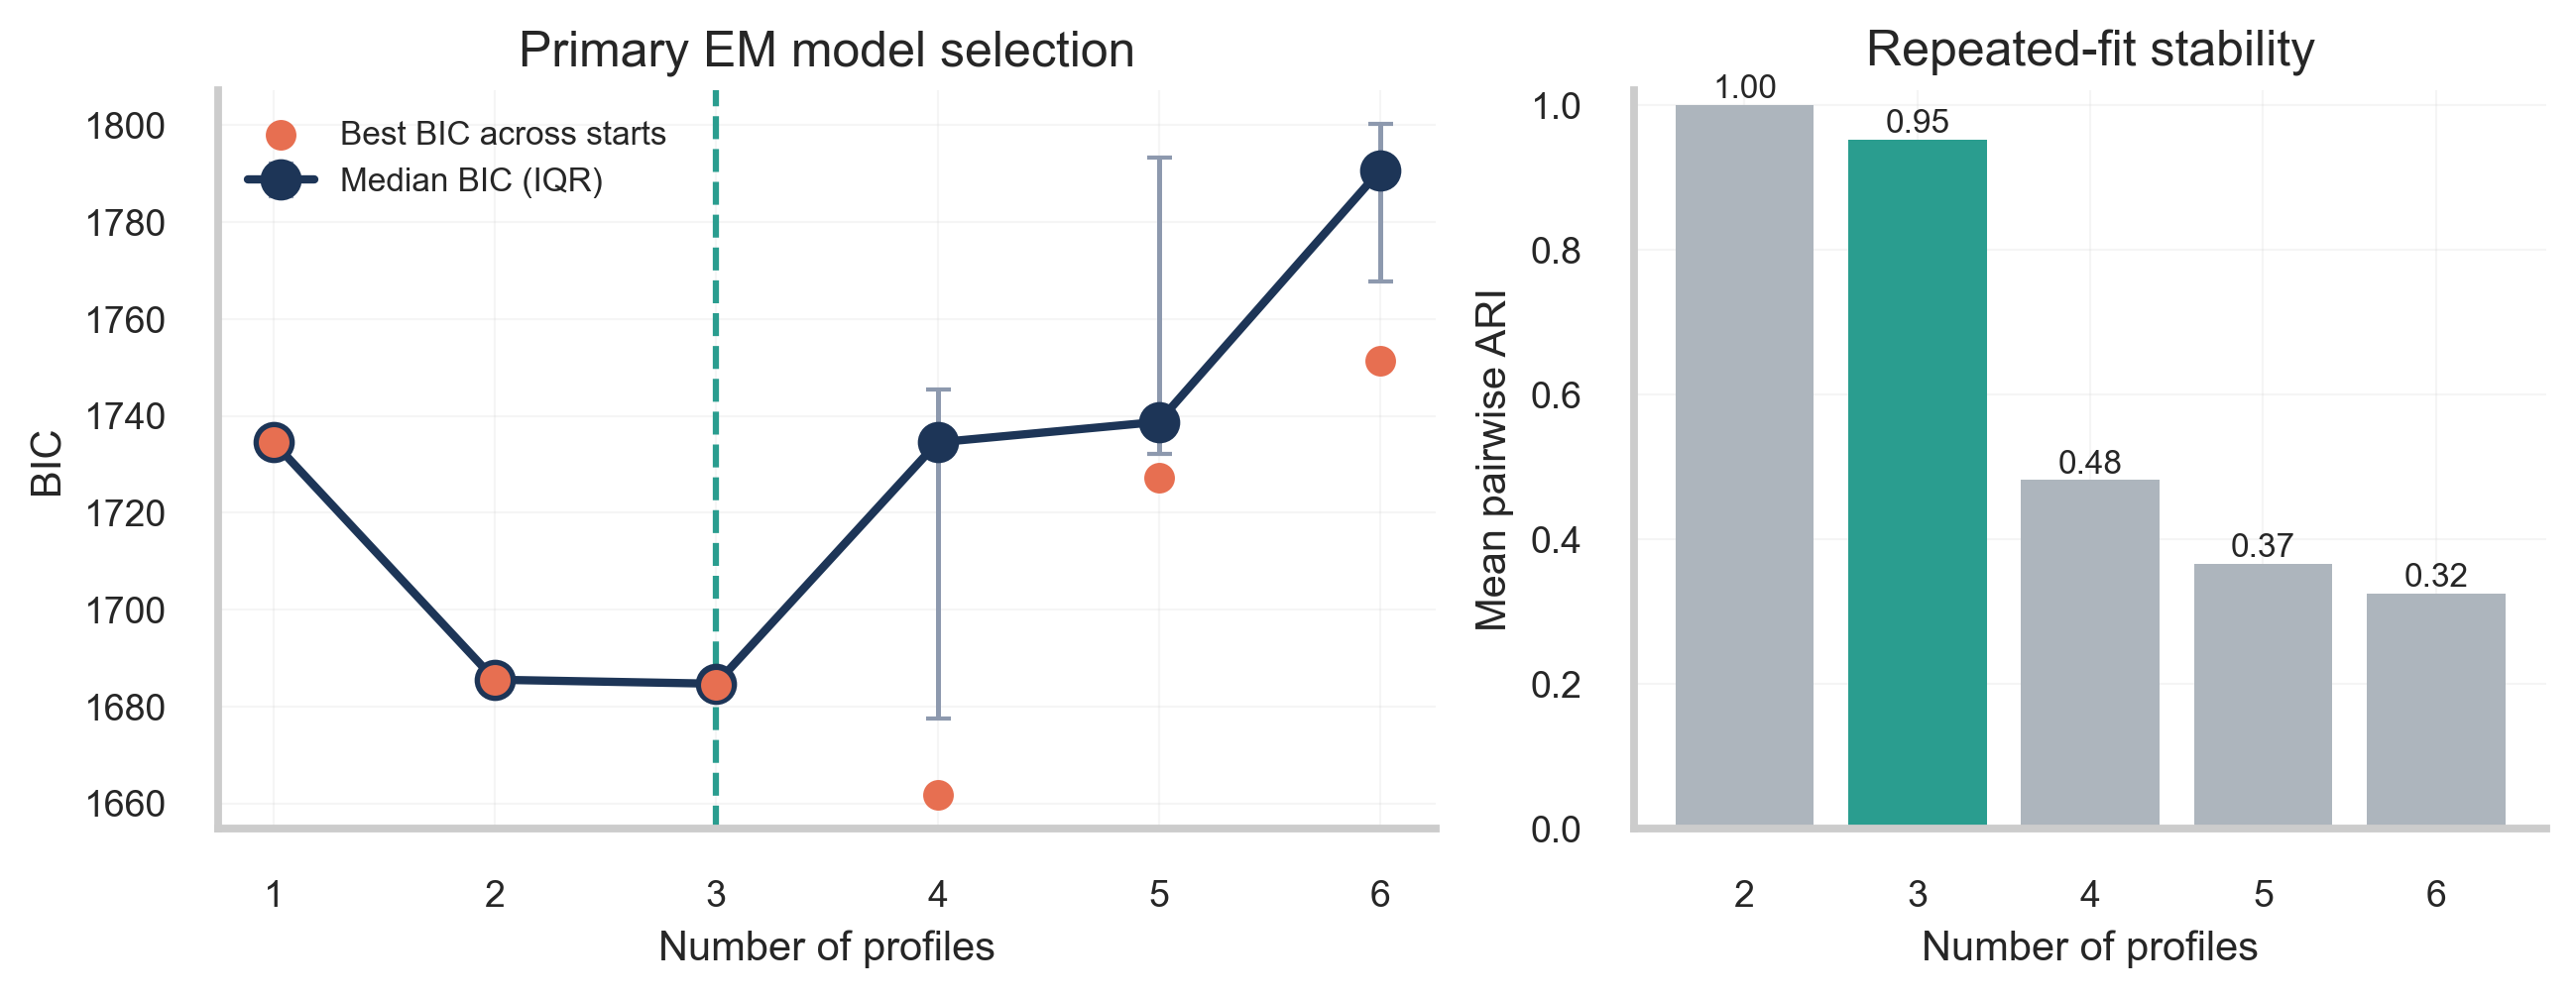
\includegraphics[width=0.93\linewidth]{../analysis_outputs/figure_8_em_extension.png}
\caption{Why the 3-profile EM solution was chosen. The 4-profile model could sometimes fit a little better, but it was much less stable across reruns.}
\label{fig:selection}
\end{figure}

\begin{figure}[H]
\centering
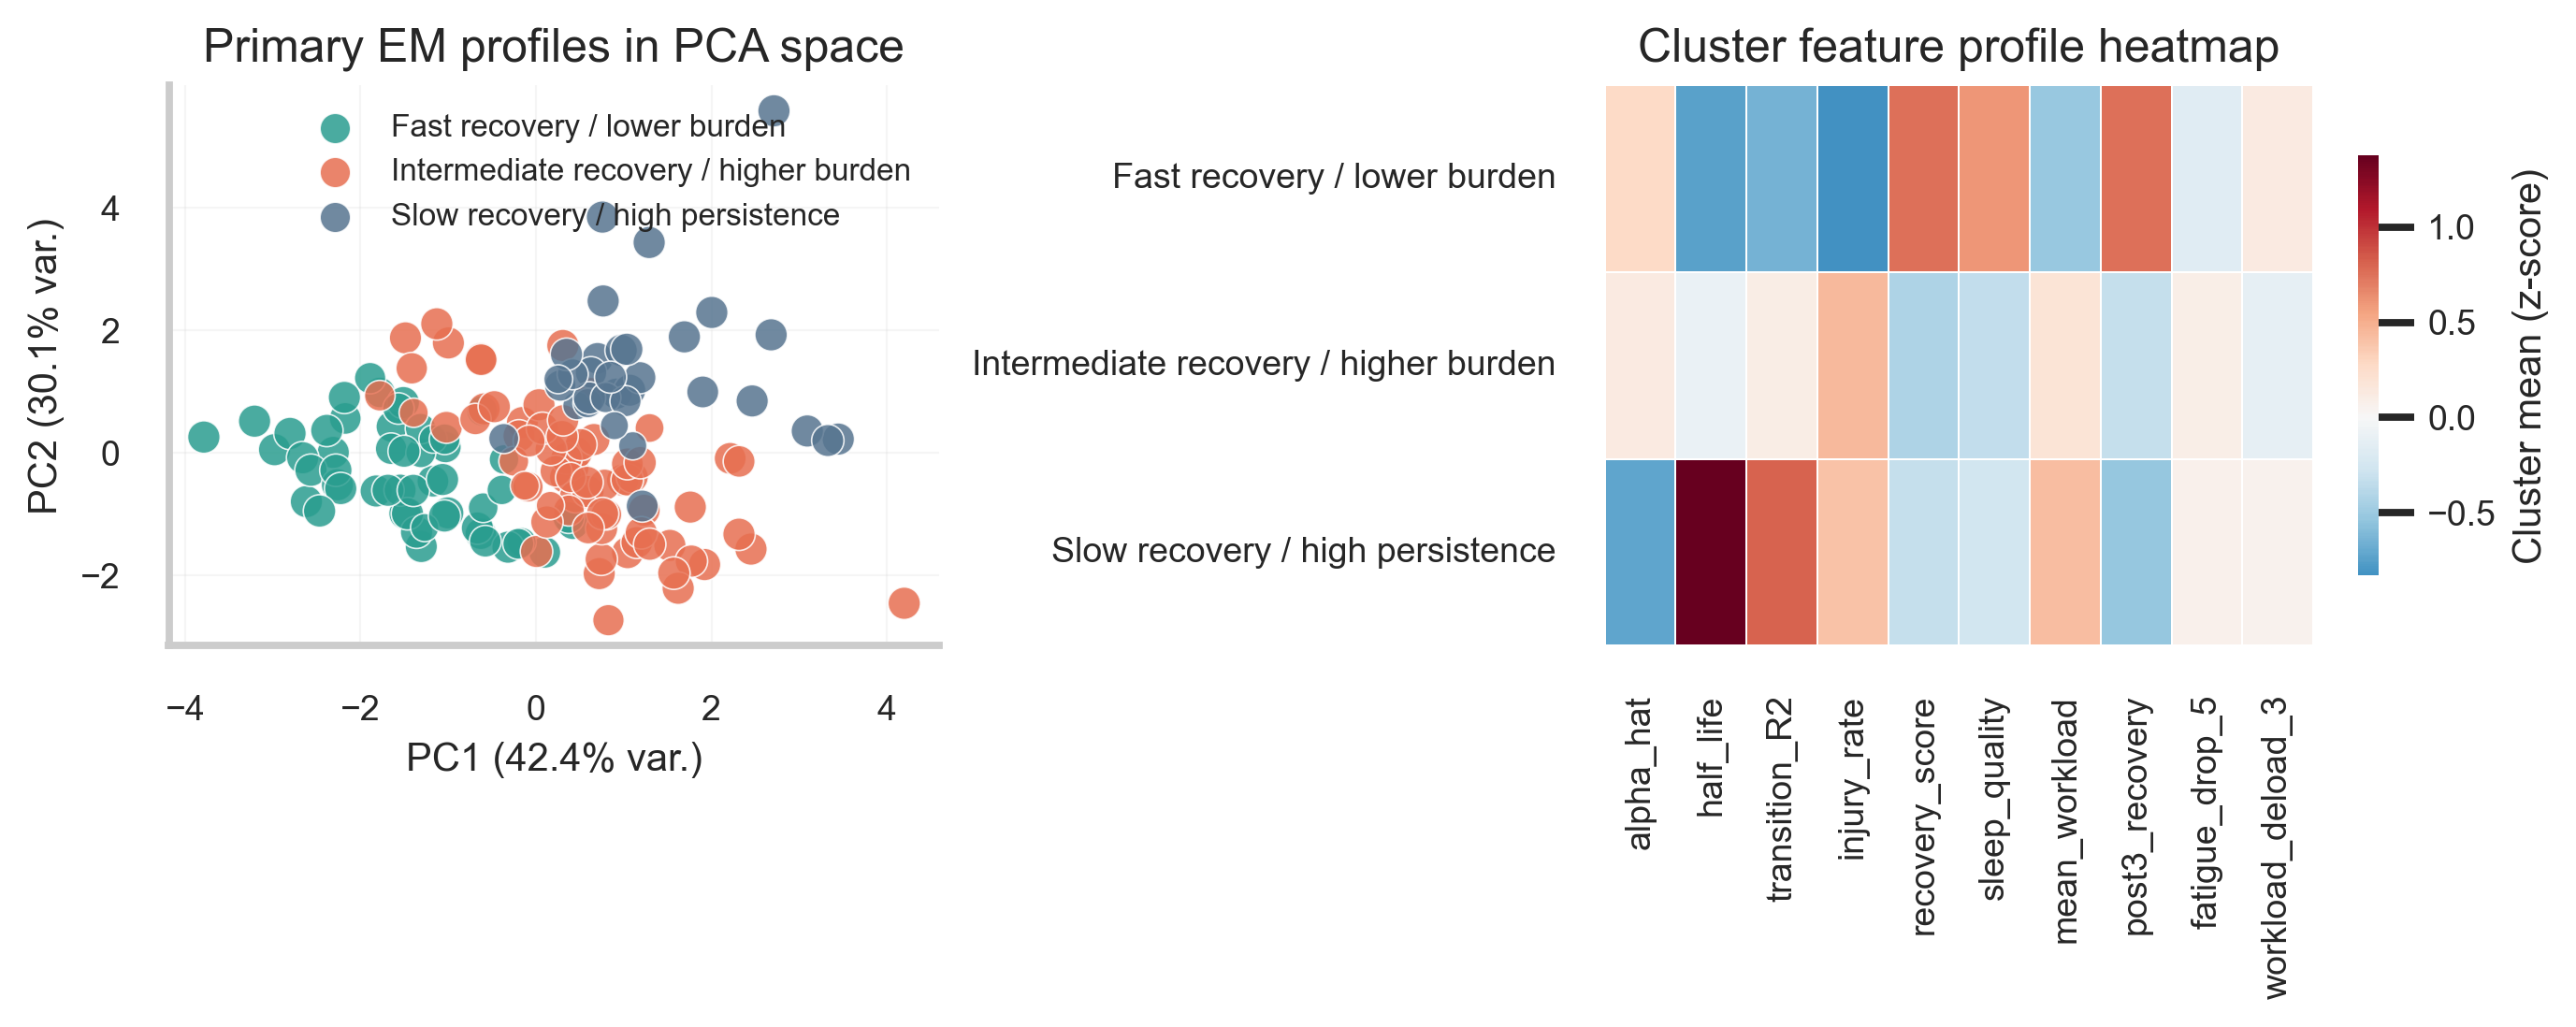
\includegraphics[width=0.93\linewidth]{../analysis_outputs/figure_8b_em_robustness.png}
\caption{What the three EM profiles look like. The left panel gives a lower-dimensional view of the athlete clusters, and the heatmap shows how the groups differ on the main recovery features.}
\label{fig:structure}
\end{figure}

\begin{figure}[H]
\centering
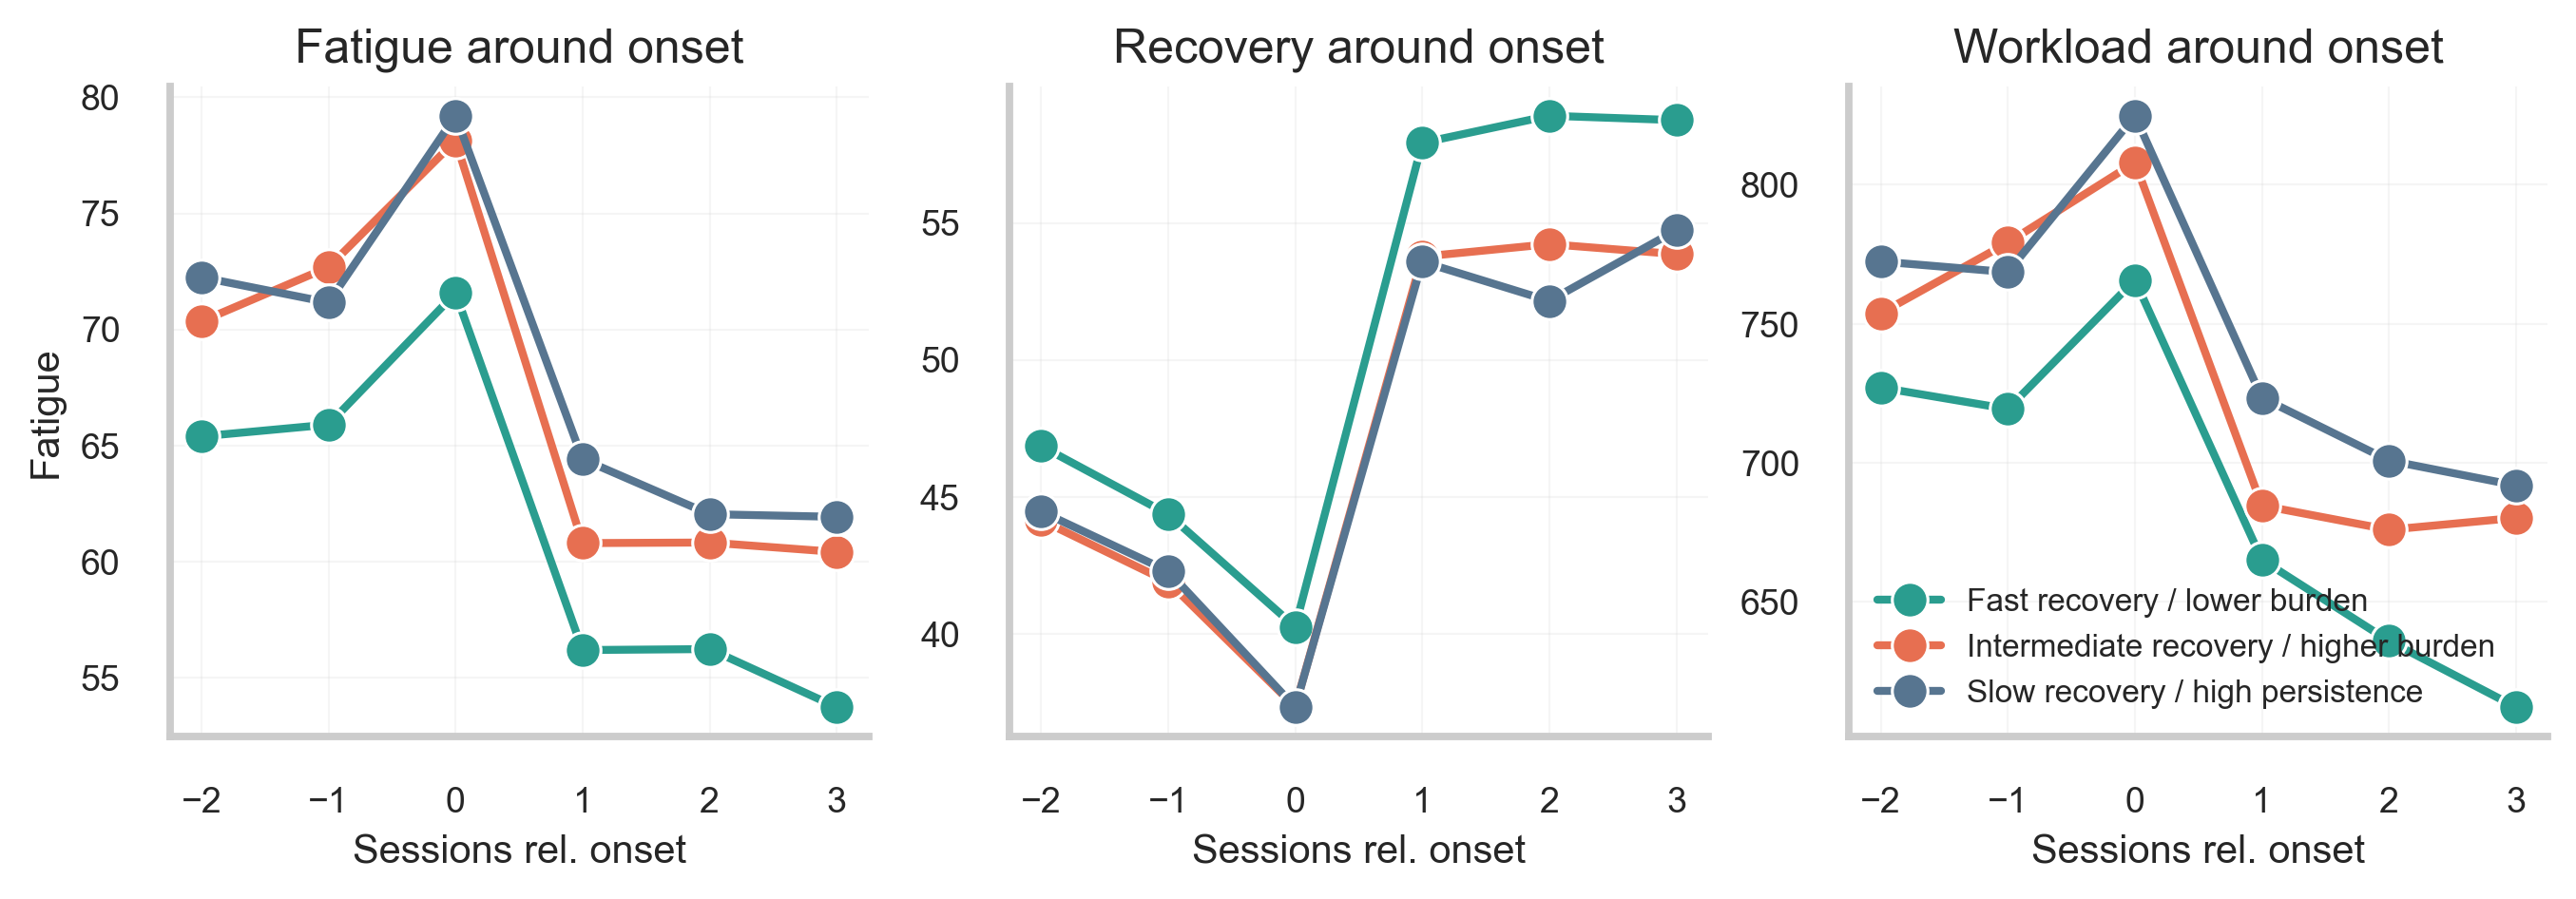
\includegraphics[width=0.93\linewidth]{../analysis_outputs/figure_8d_em_onset_profiles.png}
\caption{How the three profiles behave around injury onset. The groups differ not only in average burden, but also in how fatigue, workload, and recovery move before and after onset.}
\label{fig:onset}
\end{figure}

\begin{thebibliography}{4}
\scriptsize

\bibitem{Impellizzeri2020}
Impellizzeri, F. M., Ward, P., Coutts, A. J., Bornn, L., and McCall, A. (2020).
Training load and injury part 1: The devil is in the detail.
\textit{Journal of Orthopaedic and Sports Physical Therapy}, 50(10), 574--576.

\bibitem{Imbach2022}
Imbach, F., Sutton-Charani, N., Montmain, J., Candau, R., and Perrey, S. (2022).
The use of fitness-fatigue models for sport performance modelling.
\textit{Sports Medicine - Open}, 8, 29.

\bibitem{Dempster1977}
Dempster, A. P., Laird, N. M., and Rubin, D. B. (1977).
Maximum likelihood from incomplete data via the EM algorithm.
\textit{Journal of the Royal Statistical Society: Series B}, 39(1), 1--22.

\bibitem{Dataset2025}
Bhegam, A. (2025).
Multimodal Sports Injury Prediction Dataset.
Kaggle dataset documentation bundled with the local archive.

\end{thebibliography}

\end{document}
